\documentclass[USenglish,pdftex,compress,10pt,svgnamesi,handout]{beamer}
%\documentclass[USenglish,pdftex,compress,10pt,svgnames]{beamer}
\usepackage{import}\subimport{../../common/}{lectureheader}

\graphicspath{{pics/}}
\usepackage{listings}

\parskip2ex
\usepackage{tabu}

\newcommand{\bfw}{\Vec{w}}
\newcommand{\bfx}{\Vec{x}}
\newcommand{\bfz}{\Vec{z}}
\newcommand{\bfg}{\Vec{g}}
\newcommand{\bfu}{\Vec{u}}
\def\bf#1{\Vec{#1}}
\def\cl#1{{\cal #1}}
\DeclareMathOperator{\sgn}{sgn}
\def\hid{{H}}


% =====================================================================
% Titel etc.
\hypersetup{%
	pdftitle={neural networks: introduction},%
	pdfauthor={Patrick van der Smagt}%
}

\title{neural networks:  introduction}
\author{Patrick van der Smagt}
\date{}
% =====================================================================
\begin{document}
\lstset{language=Pascal}


%'''''''''''''''''''''''''''''''''''''''''''''''''''''''''
\begin{frame}
	\titlepage
	
	\vfil
\end{frame}










\begin{frame}
    \frametitle{A noisy real-valued function}
    
\begin{center}
	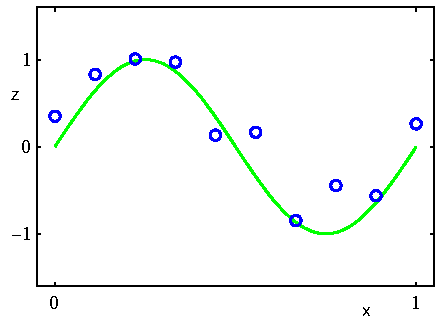
\includegraphics[width=0.7\textwidth]{pics/linreg-Figure1_2}
\end{center}
\vskip-5ex
	\begin{align}
	\text{inputs: } & \Vec{X} = (x_1,\ldots,x_N)\T\\
	\text{targets: } & \Vec{\target} = (\target_1,\ldots,\target_N)\T, \quad \target_i = h(x_i) + \epsilon = \sin(2\pi x_i)+ \epsilon
	\end{align}
\footnotesize{These figures are from C. Bishop: Pattern Recognition and Machine Learning}
\end{frame}

\begin{poll}
\begin{figure}
	\centering
	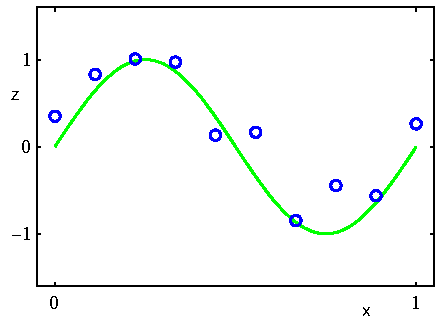
\includegraphics[width=0.6\linewidth]{pics/linreg-Figure1_2}
\end{figure}
If the green line in the plot represents the true underlying process, which problem do we encounter if we use a 9th order polynomial for linear regression?
	\begin{description}
		\item[A] curse of dimensionality
		\item[B] overfitting
		\item[C] cross validation
	\end{description}

\end{poll}
%%
\begin{frame}
    \frametitle{Model: 0th order polynomial}
    
\begin{center}
	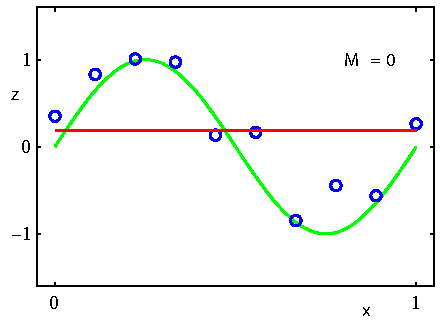
\includegraphics[width=0.7\textwidth]{pics/linreg-Figure1_4a}
	
	\alert{\[y(x,\Vec{w}) = w_0\]}
\end{center}
\end{frame}
%%
\begin{frame}
    \frametitle{Model: 1st order polynomial}
    
\begin{center}
	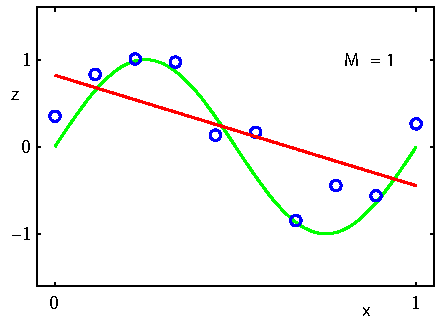
\includegraphics[width=0.7\textwidth]{pics/linreg-Figure1_4b}
	
	\alert{\[y(x,\Vec{w}) = w_0 + w_1 x\]}
\end{center}
\end{frame}
%%
\begin{frame}
    \frametitle{Model: 3rd order polynomial}
    
\begin{center}
	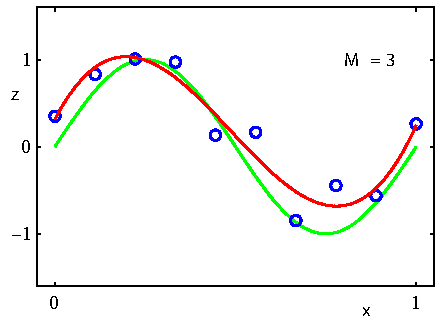
\includegraphics[width=0.7\textwidth]{pics/linreg-Figure1_4c}
	
	\alert{\[y(x,\Vec{w}) = w_0 + w_1 x + w_2 x^2 +  w_3 x^3\]}
\end{center}
\end{frame}
%%
\begin{frame}
    \frametitle{Model: 9th order polynomial}
    
\begin{center}
	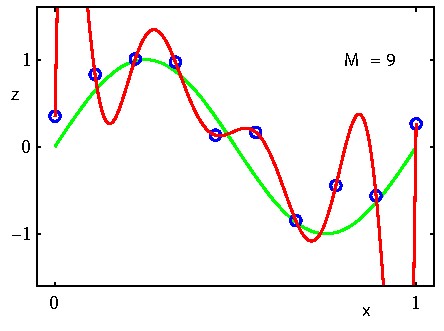
\includegraphics[width=0.7\textwidth]{pics/linreg-Figure1_4d}
	\alert{\[y(x,\Vec{w}) = \sum_{j=0}^M w_j x^j\]}
\end{center}
\end{frame}
%%
\section[LBF Models]{Linear Basis Function Models}
\subsection{Properties}
\begin{frame}
	\frametitle{Problem Definition}
	
	We have input vectors \textcolor{blue}{$\Vec{x}$} and associated
    output values \textcolor{blue}{$\target$}. We want to describe the underlying
    functional relation.
	\bigskip
\pause

What about the following simple model?
\begin{equation}
	y(\Vec{x},\Vec{w}) = w_0 + \sum_{j=1}^{M-1}w_j\phi_j(\Vec{x}) = \Vec{w}\T\Vec{\phi}(\Vec{x})
\end{equation}

where

\begin{tabular}[t]{llcl}
	$\Vec{\phi}$ & \Def{basis function} &---&  many choices, can be nonlinear\\
	$w_0$ & \Def{bias} &---& equivalent to defining $\phi_0 \equiv 1$ \\
\end{tabular}\medskip
\pause

It is \Def{linear} in $\Vec{w}$! Nothing new if you know 
Taylor expansion, Fourier transform, wavelets\dots

\end{frame}

\begin{frame}
	\frametitle{Typical Basis Functions}
\hspace{-0.8cm}\begin{tabular}{ccc}
	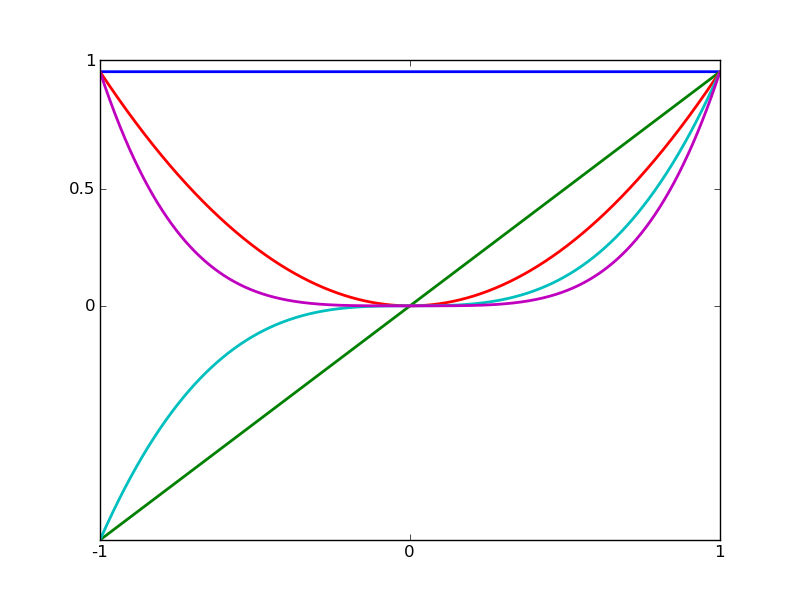
\includegraphics[width=0.32\textwidth]{pics/poly_bf.png}&
	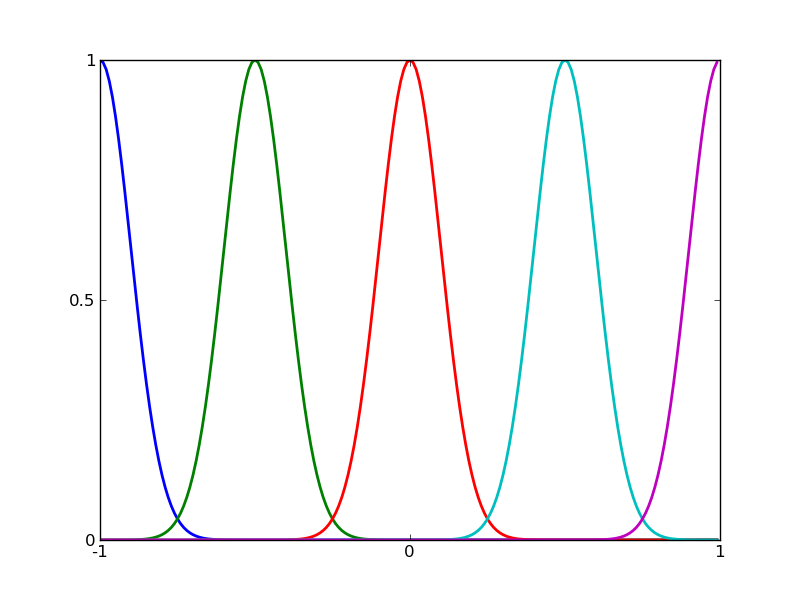
\includegraphics[width=0.32\textwidth]{pics/gauss_bf.png}&
	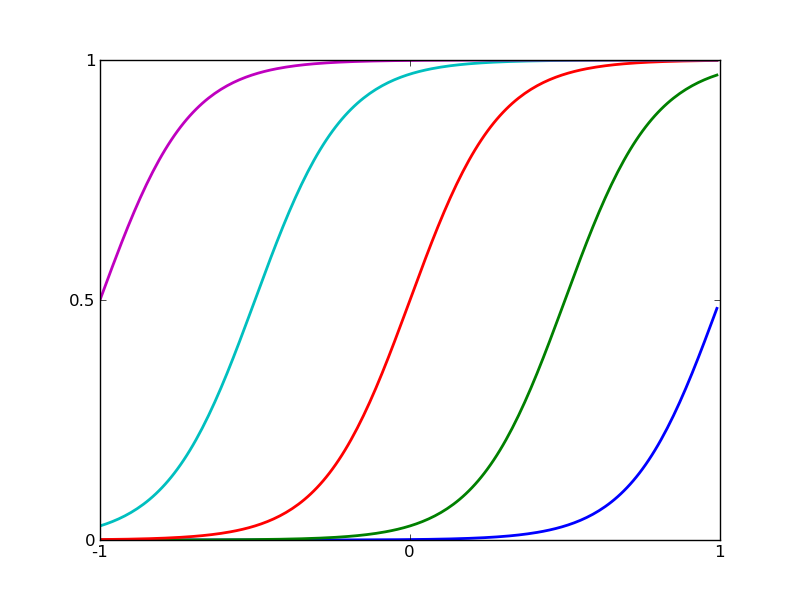
\includegraphics[width=0.32\textwidth]{pics/sig_bf.png}\\
	polynomials & Gaussians & ``sigmoids''\\
	& & (=S-shaped curves)
\end{tabular}
\end{frame}

\begin{poll}
What are the equations of the green, red, turquoise basis functions shown here?

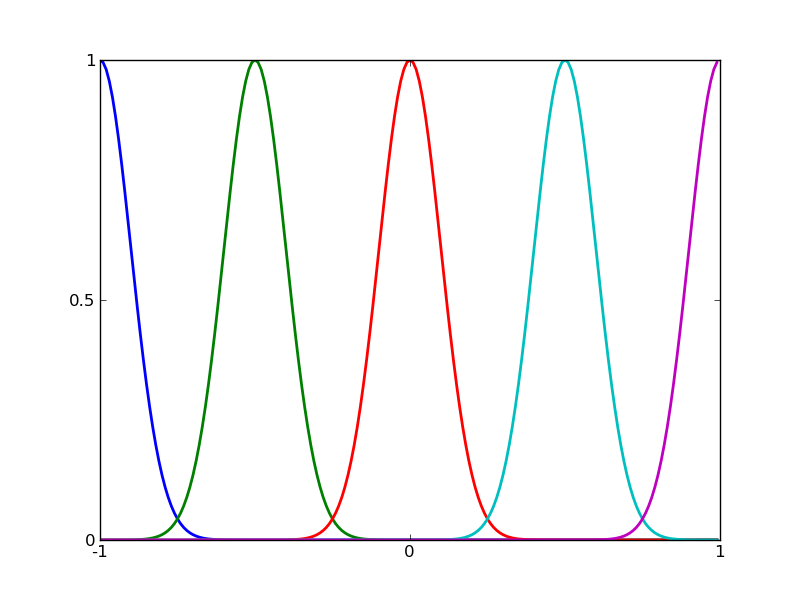
\includegraphics[width=0.6\textwidth]{pics/gauss_bf.png}

\begin{enumerate}
\item[A] $a\exp(-40x^2)$, $a\in\{-0.5, 0, 0.5\}$
\item[B] $\exp(-40(x-a)^2)$, $a\in\{-0.5, 0, 0.5\}$
\item[C]$\exp(-40(ax)^2)$, $a\in\{-0.5, 0, 0.5\}$
\end{enumerate}
\end{poll}


\begin{frame}
\frametitle{towards nonlinear systems}
How do we find optimal basis functions?

\pause
The above system could be graphically represented like this \\(this is \textsl{not} a graphical model)

\centerline{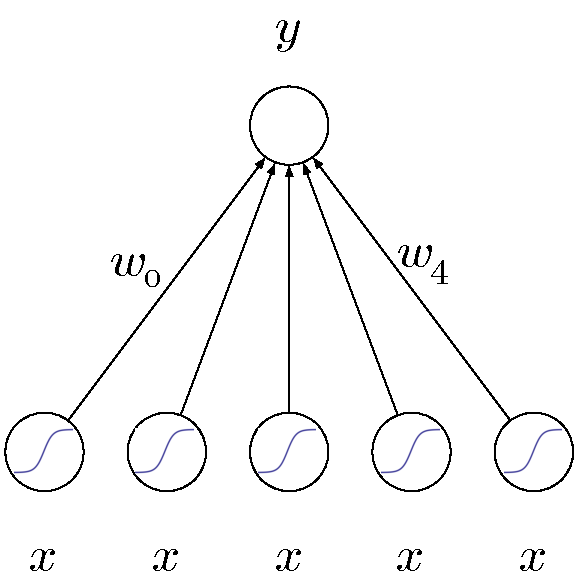
\includegraphics[width=35mm]{linreg-pict}}

where the arrows represent weights and the circles the basis functions.  

Why don't we let the system find the optimal basis functions?
\end{frame}


\begin{frame}
\frametitle{the multi-layered perceptron = neural network}
We can extend the system with an additional layer, and get

\centerline{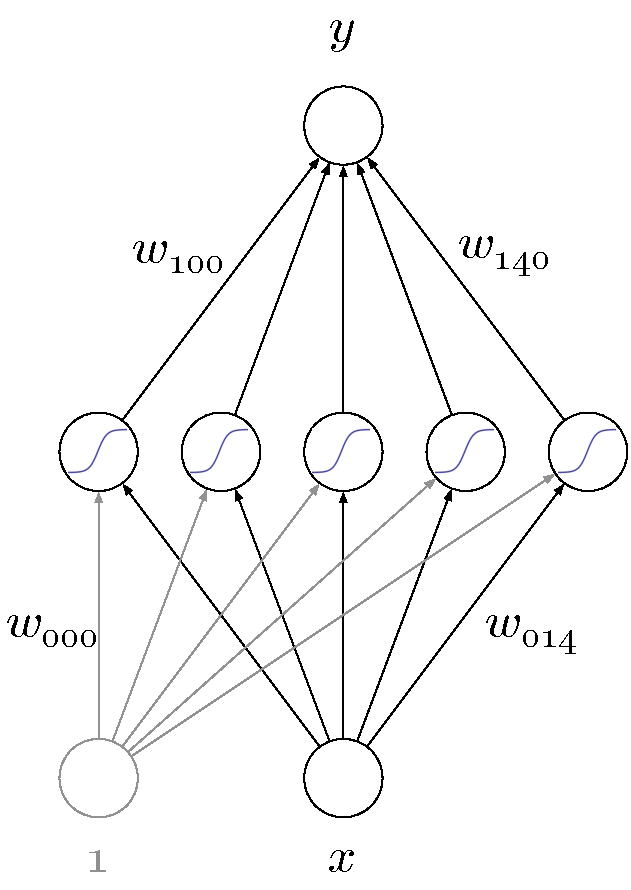
\includegraphics[width=35mm]{nn-pict}}

\resizebox{\textwidth}{!}{\hbox{(for simplicity, the constant ``1'' is usually and from now on not depicted.  But you always need it!)}}

We have generalised to
$
	y(\Vec{x},\Vec{w}_0, \Vec w_1) = \Vec{w}_1\T\Vec{\phi}(\Vec{w}_0^T\,\Vec{x})
$
\end{frame}




\begin{frame}
\frametitle{the deep neural network}
We can continue adding more hidden layers

\centerline{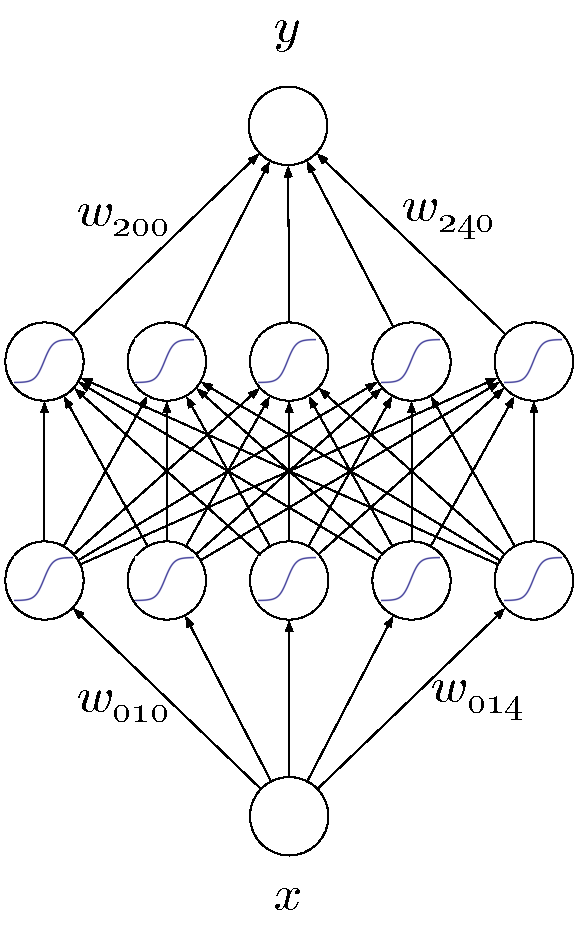
\includegraphics[width=35mm]{nn-deep-pict}}

and get a deep neural network:
$
	y(\Vec{x},\Vec{w}) =
		  \Vec{w}_2\T\Vec{\phi}\bigl(\Vec{w}_1\T\Vec{\phi}(\Vec{w}_0^T\,\Vec{x})\bigr)
$.
\end{frame}




\begin{frame}
\frametitle{how do we find $W$?}

Remember that our data set consists of targets $\Vec{\target}=(\target_1,\target_2,\ldots,\target_N)$ 
and corresponding input vectors $\Vec{X}=(\Vec{x}_1,\Vec{x}_2,\ldots,\Vec{x}_N)$.

We measure random variable  $\target$ as
\begin{equation}
	\target=y(\Vec{x},\Vec{w}) + \Vec{\epsilon} \Annot{[$\epsilon$: Gaussian, zero mean]}
\end{equation}

Then the \Def{log likelihood} is
\begin{equation}\label{eqn:likelihood}
  \ln p(\Vec{\target}\mid \Vec{X},\Vec{w}) \propto
    -{1\over2} \sum_{n=1}^N \bigl(\target_n - y(\Vec x_n, \Vec w)\bigr)^2
\end{equation}

We call the negative log likelihood the \Def{loss} ${\cal L}(\Vec w)$ aka $E(\Vec w)$.
\end{frame}



\begin{frame}
\frametitle{how do we find $W$?}
In the maximum-likelihood solution we therefore minimise
$$E = \sum_{n=1}^N \bigl(\target_n - y(\Vec x_n, \Vec w)\bigr)^2$$

There is one difference w.r.t.\ linear regression: $E(\Vec w)$ is no longer convex!

How can this be minimised?  The minimum is located where its gradient is 0.
So one typically minimises by using the gradient:
$$\bfw_{i+1} = \bfw_i - \alpha \nabla E$$

How do we compute the gradient $\nabla E$?  
Back propagation does this.
\end{frame}



\begin{frame}
\frametitle{one slide on back-propagation}

A general rule to optimally find the weights $\bfw$ was not discovered until 1974 (Paul Werbos) or 1985 (LeCun) and 1986 (Rumelhart \textsl{et al.}): \\\textbf{back propagation}.

\vskip5mm

The idea: you need to compute the gradient $\partial E / \partial w_{ijk}$.  To do so, compute the residual $y-z$ at the output, and propagate that back the the neurons in the layers below.
From that you can then compute the gradient.

\vfill
\end{frame}


\begin{frame}[fragile]
\frametitle{algorithm for backprop (``on-line'' aka ``stochastic'' learning)}

\begin{beamerboxesrounded}[upper=def,lower=block body,width=1.03\textwidth,shadow]{\textbf{back-propagation algorithm:}}
\begin{lstlisting}[mathescape]
initialise the weights
repeat
  for each training sample $(\bfx,\bfz)$ do
  begin
    compute $\bf o = y(\bfw, \bfx)$ (forward pass)
    calculate residual $\delta_{kj} = \bfz  - \bf o$ at the output units
    for all k:
     propagate $\delta_{kj}$ back one layer by $\delta_{k-1,i} = \sum_j\delta_{kj} w_{k-1,i,j}$
    update the weights using $\partial E / \partial w_{kij} = \delta_{kj} \,\phi'(\cdot)\, x_{i}$
  end
  (this is called one epoch)
until stopping criterion satisfied
\end{lstlisting}
\end{beamerboxesrounded}
\end{frame}

\end{document}





\begin{frame}
\end{frame}



%%%%%%%%%%%%
%%%%%%%%%%%%
%%%%%%%%%%%%
%%%%%%%%%%%%
%%%%%%%%%%%%
%%%%%%%%%%%%
%%%%%%%%%%%%
%%%%%%%%%%%%
%%%%%%%%%%%%
%%%%%%%%%%%%


\begin{frame}
\frametitle{how to reduce $E$}
In the optimisation class, we dealt with many ways to optimise the error:
\begin{itemize}
\item momentum
\item flexible step width, bold driver
\item Langevin updating, Manhattan backprop, RProp, quickprop
\end{itemize}

\imgcrop{all_algorithms}{}{0.6\textwidth}{16 16 304 208}
\end{frame}


%\begin{frame}
%\frametitle{Hessian-free optimisation}
%Ideally, we reduce the error $E$ by following $\Vec w$ using Newton's method: 
%$$\Vec w \leftarrow \Vec w - H^{-1}  \nabla E$$
%where $u = H^{-1} \nabla E$ is the search direction.  We are trying to find $u$.  
%\pause
%We can compute $\nabla E$, but computing $H$ costs $O(N^2)$, $H^{-1}$ costs $O(N^3)$.
%
%Hessian-free optimisation uses the following trick:  $u = H^{-1} \nabla E$ solves to
%$$ H u = \nabla E$$
%We can find $p$ by solving
%$$  \| Hu - \nabla E\| = 0 $$
%where a method (Pearlmutter 1994 has a better one) to compute $Hu$ is
%$$ Hu = \lim_{\varepsilon \rightarrow 0} {\nabla E(\Vec w+\varepsilon) - \nabla E(\Vec w)\over \varepsilon}$$
%\end{frame}
\begin{frame}
\frametitle{Hessian-free optimisation}
Normal second-order optimisation methods require the computation of the Hessian or of its inverse (Newton methods), or at least an approximation thereof (quasi-Newton methods).  The cost of this computation as well as of its storage is high, as $H$ is quadratic in the number of parameters (weights) of the neural network.

It appears that we can do the same by not computing $H$ but rather computing $H\bfu$ where $\bfu$ is the search direction.  That is only a vector!

The next slide quickly explains the maths behind.
\end{frame}


\begin{frame}
\frametitle{Hessian-free optimisation }
Let us look at the 2nd-order Taylor approximation to the error around $\bfw_0$
$$
E(\bfw) 
=  E(\bfw_0) - \nabla E(\bfw_0) (\bfw - \bfw_0) + (\bfw - \bfw_0)^T H(\bfw_0) (\bfw - \bfw_0)
$$
A minimum is encountered where $\nabla E(\bfw)=0$, i.e.,
$$-\nabla E(\bfw_0) + (\bfw - \bfw_0) H(\bfw_0) = 0$$
or, when writing $\bfu=\bfw - \bfw_0$,
\begin{equation}\label{eq:HF} \bfu = H^{-1}(\bfw_0)\nabla E(\bfw_0) \end{equation}
Computing $\bfu$ using (\ref{eq:HF}) is Newton's method.  But it involves computing $H^{-1}$ which costs $O\bigl((\#w)^3\bigr)$.
Instead we define the optimal $\bfu$ as
\begin{equation}\label{eq:HFopt}
\bfu_{\mathrm{opt}} = \argmin_{\bfu} \| H(\bfw_0) \bfu - \nabla E(\bfw_0) \|
\end{equation}
We can compute the first term using finite differences:
\begin{equation}
H(\bfw_0) \bfu \approx \lim_{\epsilon \rightarrow 0} {
	\nabla E(\bfw_0 + \epsilon \bfu) - \nabla E(\bfw_0) \over \epsilon}
\end{equation}
Now we can find $\bfu$ by optimising Eq.~(\ref{eq:HFopt}) using, e.g., linear CG.
\end{frame}


\frame{\frametitle{options for regularising neural networks}
\begin{tabular}{ll}
	\textbf{Modification} & \textbf{Issues} \\\hline
	use \alert{small enough} network & $\ominus$ loses generalisation capabilities\\[2mm]
	\pause
	early stopping & $\ominus$ need extra data for testing\\
	& $\ominus$ which data to choose for cross-validation?\\[2mm]
	\pause
	introduce \alert{weight decay} term & $\ominus$ weights are regularised towards 0!\\[2mm]
	add Gaussian noise to inputs & $\ominus$ is it realistic?  \\
	& $\ominus$ increases training time\\[2mm]
	\pause
	full Bayesian treatment & $\ominus$ nonlinear transfer functions prohibit that
\end{tabular}
}



%\frame{\frametitle{choosing the best hidden layer size $N_{h}$}
%Just like in generalised linear regression, for a typical toy problem we may get something like this:
%\bigskip
%
%\begin{center}
%	\includegraphics[width=0.33\textwidth]{pics/Figure5_9a.pdf}
%	\includegraphics[width=0.33\textwidth]{pics/Figure5_9b.pdf}
%	\includegraphics[width=0.33\textwidth]{pics/Figure5_9c.pdf}
%\end{center}
%
%\begin{columns}
%\begin{column}{6cm}
%\pause
%Methods exist (Barron, 1991; Vysniauskas, 1993) which estimate the optimal number
%of hidden units $N_{h}$ and number of samples $p$ by fitting the approximation error $E$ as
%$$
%  E(p, N_h) \approx  \sum_{p} \sum_{i+j=p} {\gamma_{ij} \over p^i N_{h}^j}
%\ee  
%\end{column}
%\begin{column}{4cm}
%\includegraphics[width=4cm]{pics/minimal-resources}
%\end{column}
%\end{columns}
%}


\frame{\frametitle{weight decay}
\ParBeg{recap:} in Bayesian linear regression, assuming a Gaussian prior for the weights $\Vec{w}$ lead to a quadratic regularisation term in the log likelihood. 
\medskip

Exactly the same happens with MLPs.

Here this procedure is called \alert{weight decay}:
$$
E = \frac{1}{2} \sum_{n} \Norm{\cl M(\Vec{x}_n,\Vec{w})-\Vec{z}_n}^2 + \alert{\frac{\lambda}{2}\Vec{w}\T\Vec{w}}
$$

Minimisation of $E$ leads to our MAP solution $\Vec{w}_\text{MAP}$.

}

\frame{\frametitle{early stopping}
early stopping is probably the most widely used regularisation technique for MLPs. 
  \begin{columns}[T]
    \begin{column}{0.50\textwidth}
\imgbox{bias+variance}{Bias-variance dilemma}{\textwidth}
    \end{column}
    \begin{column}{0.50\textwidth}
\imgcrop{overtraining}{Real-world example}{\textwidth}{15 15 264 208}
    \end{column}
  \end{columns}\bigskip

\ParBeg{Note:} In typical applications, use about 10\% to 25\% of the data for testing.  Equivalence to weight decay can be argued.
}

%\frame{\frametitle{early stopping and weight decay}
%A typical training algorithm follows the steepest gradient first, starting with weights near zero:
%
%\includegraphics[width=0.45\textwidth]{pics/Figure5_13.pdf}\hfill
%\includegraphics<2->[width=0.45\textwidth]{pics/Figure3_15.pdf}
%
%\onslide<2-> 
%We follow a trajectory in weight space and stop at $\widetilde{\Vec{w}}$, when the validation set tells us so. 
%In effect, this moves the weight to $\widetilde{\Vec{w}}$ along an ev of $\nabla^2E$ with small ev. The increase in $E$ is small but the decrease in $|\bfw|$ large!
%
%This is approximately the same location as $\Vec{w}_\text{MAP}$! With learning rate $\alpha$ and iteration $t$, it can be shown (under some conditions) that
%\alert{$\alpha t \propto \lambda^{-1}$}.
%
%}











\begin{frame}
\frametitle{some good and some bad news}
\hfill
\begin{beamerboxesrounded}[scheme=proof,width=0.95\textwidth,shadow=true]{\textbf{universal approximation}}
	an MLP with at least two layers of weights can approximate arbitrarily well any given mapping from one finite input space with a finite number of discontinuities to another, if we have enough hidden units [Cybenko 1989; Funahashi 1989; Hornik et al 1989, 1991; Hartman et al 1990].
\end{beamerboxesrounded}
\hspace*{\fill}
\bigskip
	\pause

\hfill
\begin{beamerboxesrounded}[scheme=proof,width=0.95\textwidth,shadow=true]{\textbf{parameter finding}}
	finding the optimum set of weights $\bfw$  for an MLP is an NP-complete problem, i.e.\ it cannot be solved exactly within a time $t\propto |\bfw|^x$ [Blum et al., 1992].
\end{beamerboxesrounded}
\hspace*{\fill}
\end{frame}


\begin{frame}
\frametitle{the name of the game}

feed-forward neural network (FFNN), neural network, multi-layer perceptron (MLP)

back-propagation (BP), backprop, generalised delta rule

\pause
FFNN's have been used in many areas, including process control, classification, stock exchange prediction, diagnosis, robot control, sensory data fusion, etc. But they did not live up to their expectation, and after their hype (1986--1995) they lost in popularity.  

In fact, their restricted representation and generalisation properties was one of the biggest problems.

$\rightarrow$ IEEE journals, ICML had policies not to accept NN papers

%Recent results have shown that the don't-give-up approach can give great results; a new hype (2010--) shows
%that they can be used to solve real-world problems (allegedly Siri, Street View house number recognition, speech recognition, image recognition, \dots)
\end{frame}


\begin{frame}
\frametitle{why did the multi-layered perceptron not get popular?}
\vskip5mm
\centerline{\includegraphics[width=6cm]{pics/ffnn.png}}

\begin{eqnarray*}
 \cl M (\bfw, \bfx) &=& \sum_{i^{(\hid)}} w^{(\hid)}_{i^{(\hid)}} \phi \left(\sum_{i^{(\hid-1)}=1}^{N_{\hid-1}} w^{(\hid-1)}_{i^{(\hid)},i^{(\hid-1)}} 
 		\phi\left( \sum_{i^{(\hid-2)}=1}^{N_{\hid-2}} w^{(\hid-2)}_{i^{(\hid-1)},i^{(\hid-2)}} \right.\right.
		\cdots\\
		&&
 		\cdots\left.\left.\phi\left( \sum_{i^{(1)}=1}^{N_{1}=d} w^{(1)}_{i^{(2)},i^{(1)}}
		x_{i^{(1)}} \right)\right)\right)
\end{eqnarray*}
\end{frame}


% use this for invisible text, in particular invisible underbraces
\def\i#1{\textcolor{white}{#1}}

%% vanishing gradient
\begin{frame}<handout:0>
\frametitle{a big problem: the vanishing gradient}
It is usually true that 
$$  \partial E(\bfw) / \partial w_{ij}^{(\hid)}
  \gg
    \partial E(\bfw) / \partial w_{ij}^{(\hid-1)}
$$
i.e., the lower you get in the network, the more the gradient vanishes.

After all,
$$
{\partial E(\bfw)  \over \partial w_{ij}^{(\hid-1)} }
    = \delta^{(\hid-1)}_j x_i 
    = \sum_l \i{\underbrace{\textcolor{black}{\delta_l^{(\hid)}}}_{\mathrm{small}}}
    	\i{\underbrace{{}_l^(}_{\i{\times}}}
	\i{\underbrace{ \textcolor{black}{w_{lk}^{\i(} x_i }}_{\mathrm{small}}}
	\i{\underbrace{=smaller_l^(}_{=\,\,\,\mathrm{smaller!}}} 
$$\end{frame}

\begin{frame}
\frametitle{a big problem: the vanishing gradient}
It is usually true that 
$$  \partial E(\bfw) / \partial w_{ij}^{(\hid)}
  \gg
    \partial E(\bfw) / \partial w_{ij}^{(\hid-1)}
$$
i.e., the lower you get in the network, the more the gradient vanishes.

After all,
$$
{\partial E(\bfw)  \over \partial w_{ij}^{(\hid-1)} }
    = \delta^{(\hid-1)}_j x_i 
    = \sum_l {\underbrace{\textcolor{black}{\delta_l^{(\hid)}}}_{\mathrm{small}}}
    	\i{\underbrace{{}_l^(}_{\textcolor{black}{\times}}}
	{\underbrace{ \textcolor{black}{w_{lk}^{\i(} x_i }}_{\mathrm{small}}}
	\i{\underbrace{=smaller_l^(}_{\textcolor{black}{=\,\,\,\mathrm{smaller!}}}}
$$\end{frame}







\begin{frame}
\frametitle{$E($XOR$)$, 1 hidden layer}
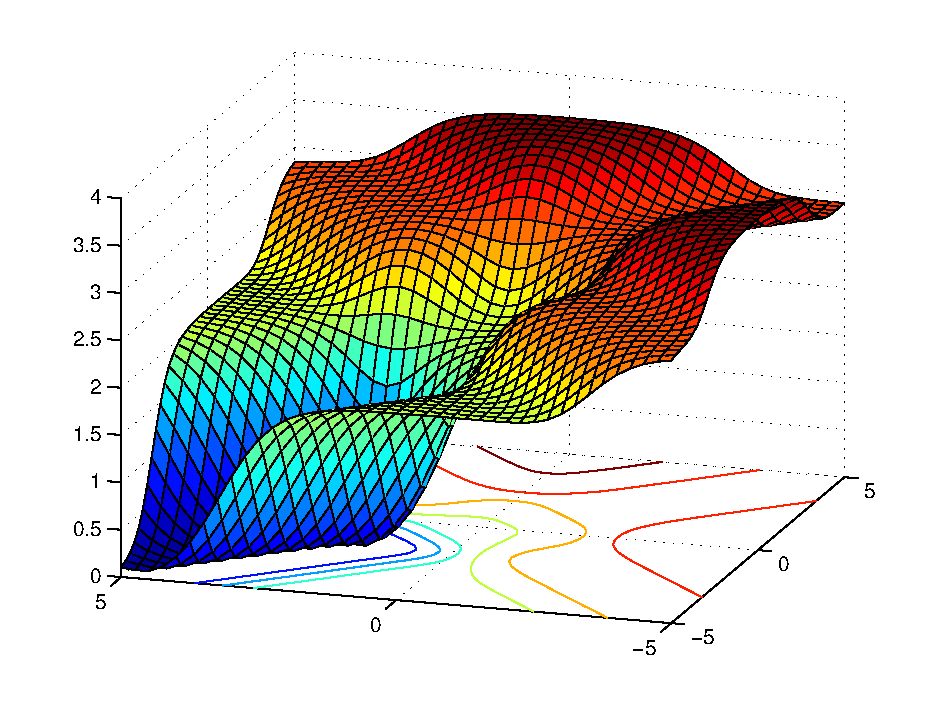
\includegraphics[width=6cm]{pics/xor_in1_1hidden}
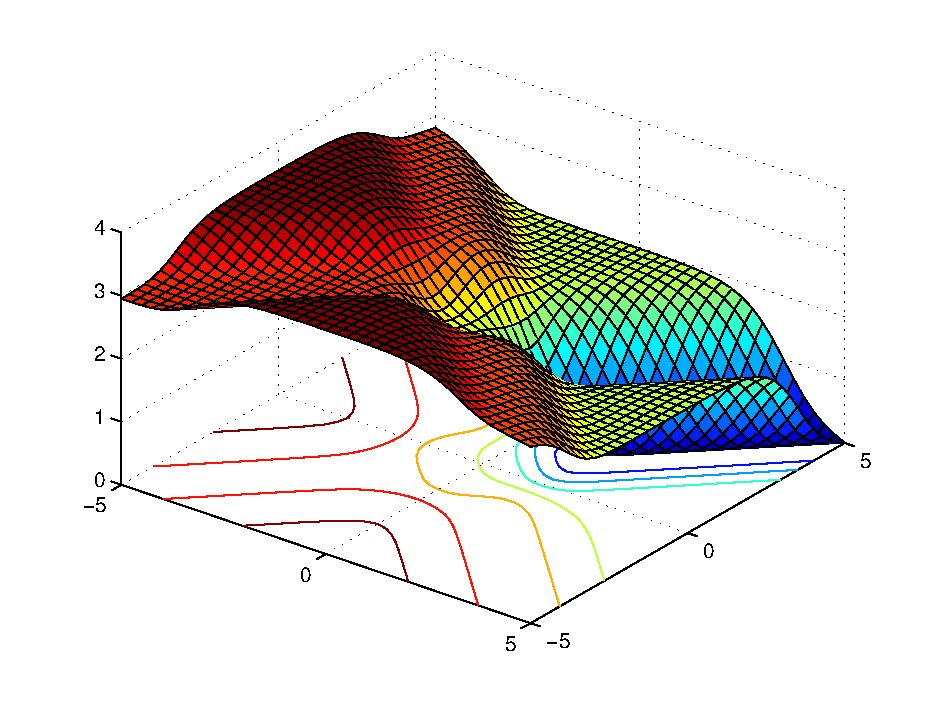
\includegraphics[width=6cm]{pics/xor_in2_1hidden}

$E(w^{(1)})$
\end{frame}



\begin{frame}
\frametitle{$E($XOR$)$, 3 hidden layers}
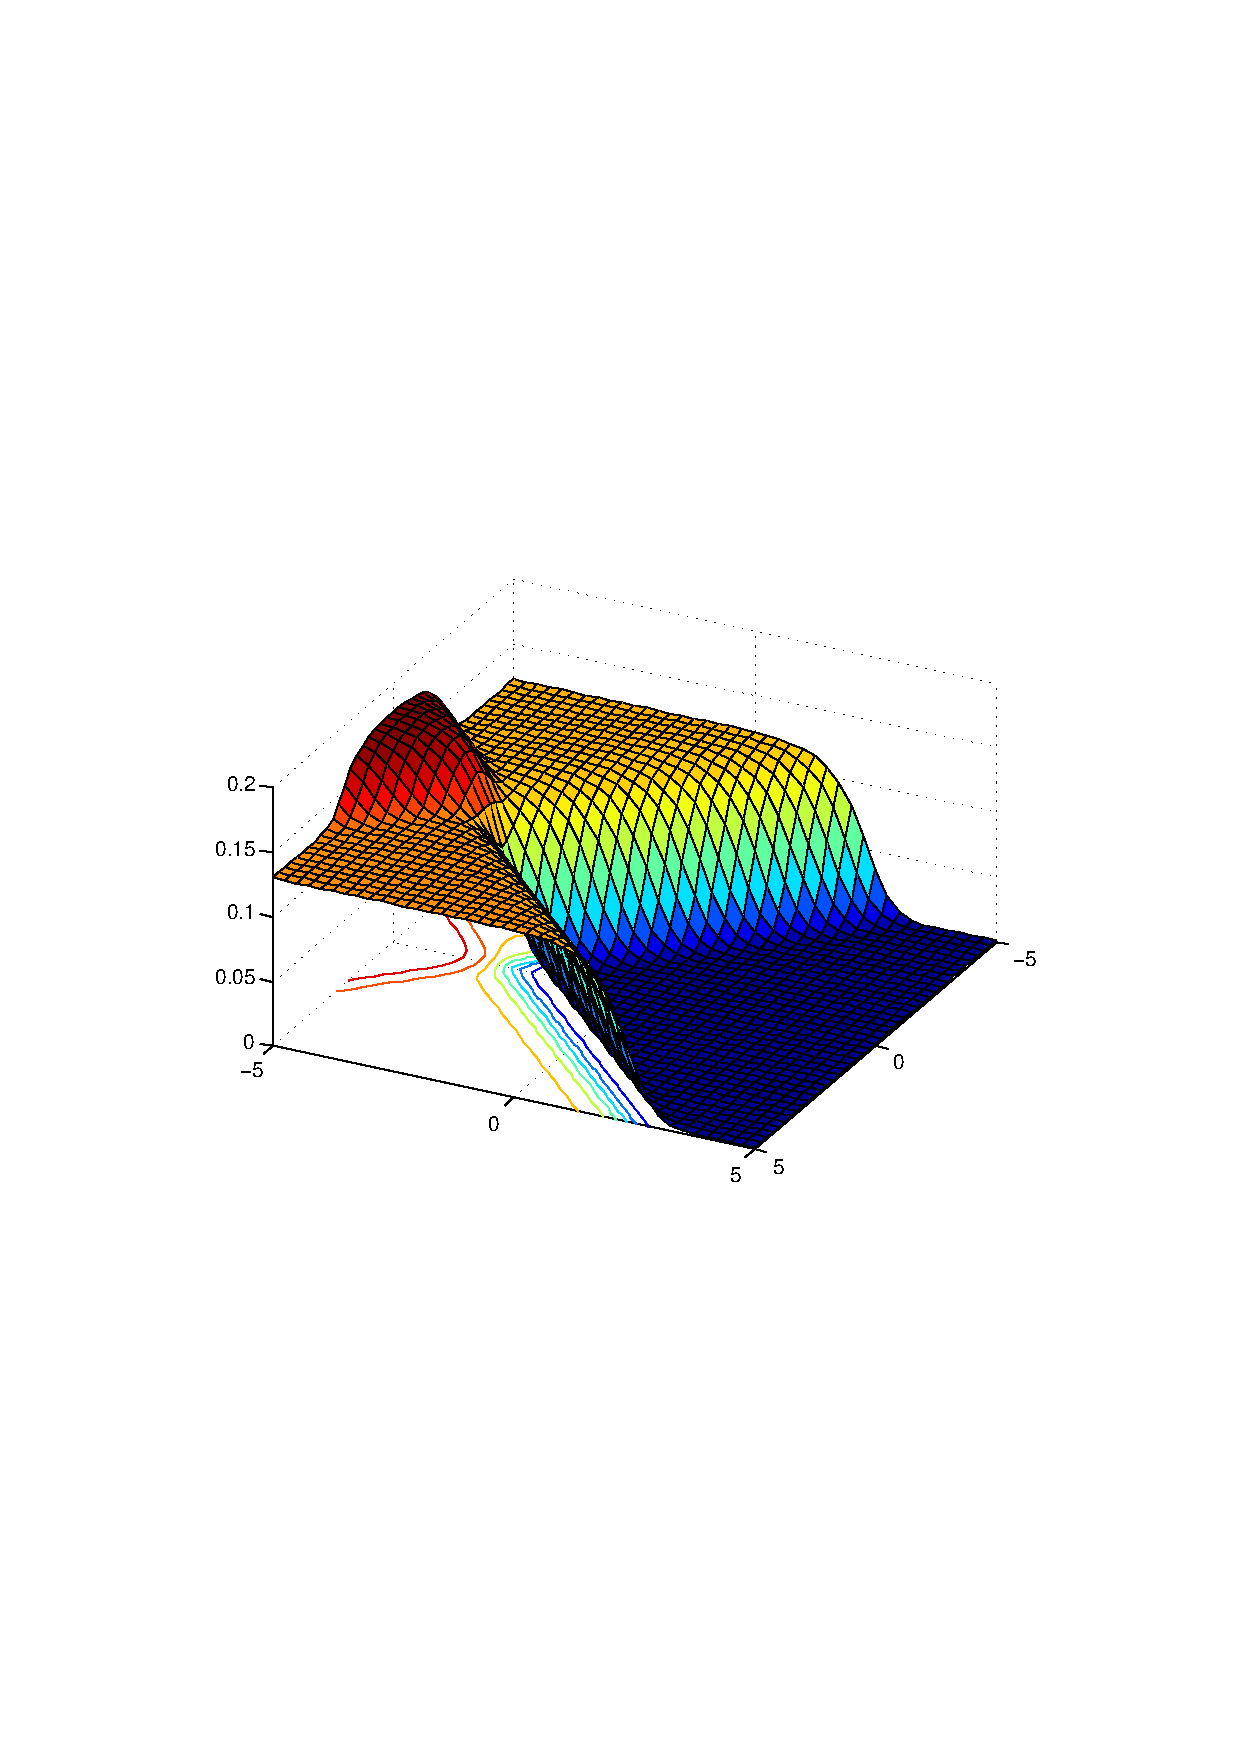
\includegraphics[width=6cm]{pics/xor_in1_3hidden}
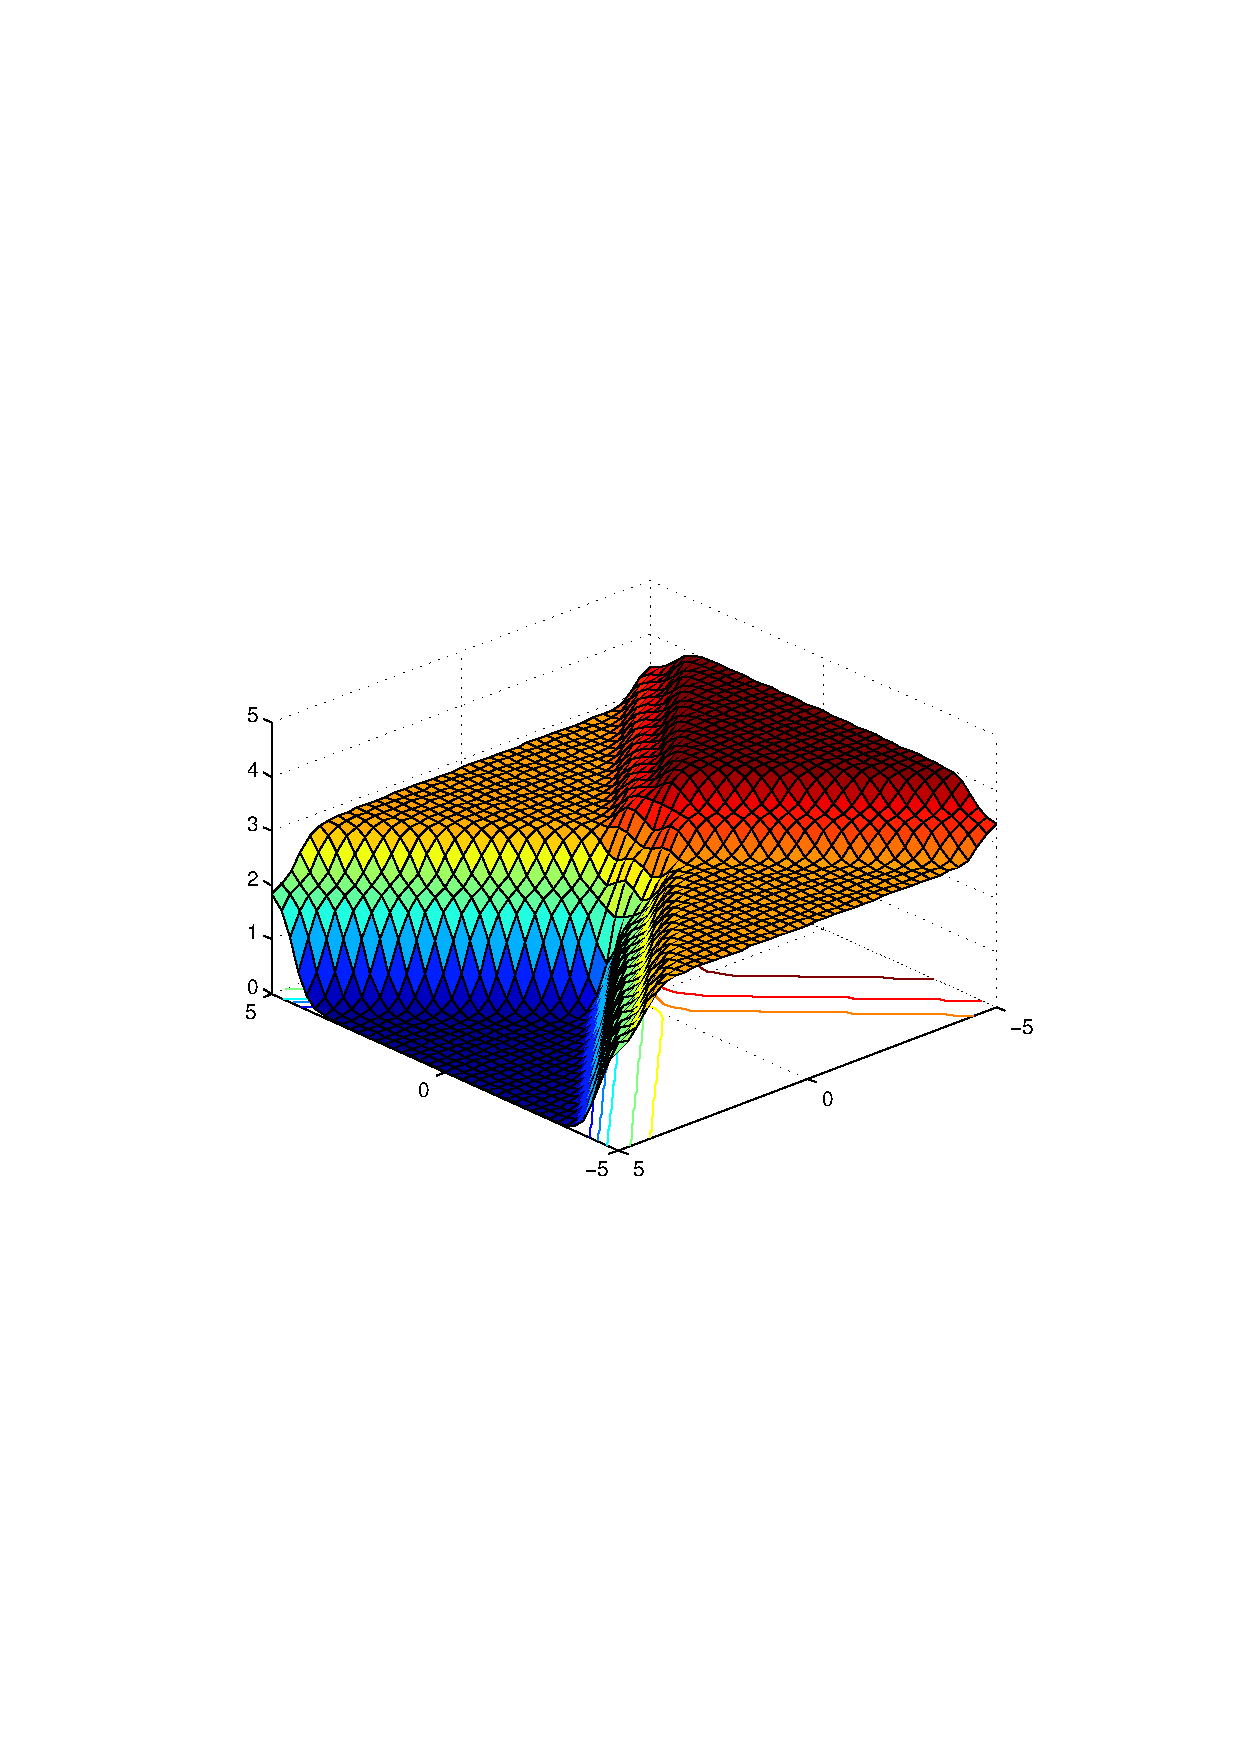
\includegraphics[width=6cm]{pics/xor_in2_3hidden}

$E(w^{(1)})$
\end{frame}


\begin{frame}
\frametitle{$E($XOR$)$, 10 hidden layers}
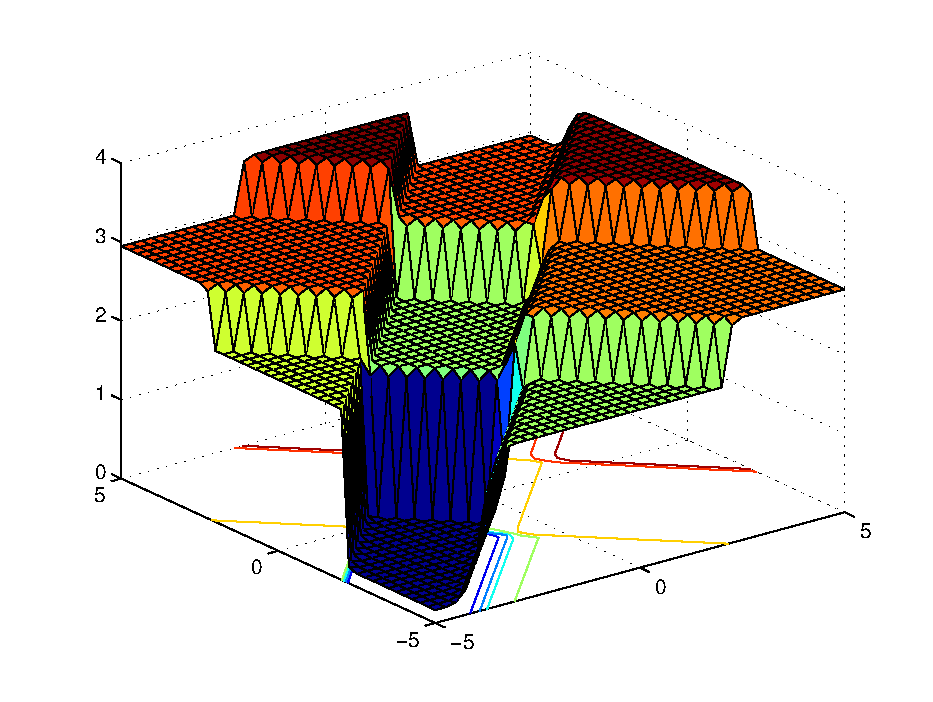
\includegraphics[width=6cm]{pics/xor_in1_10hidden}
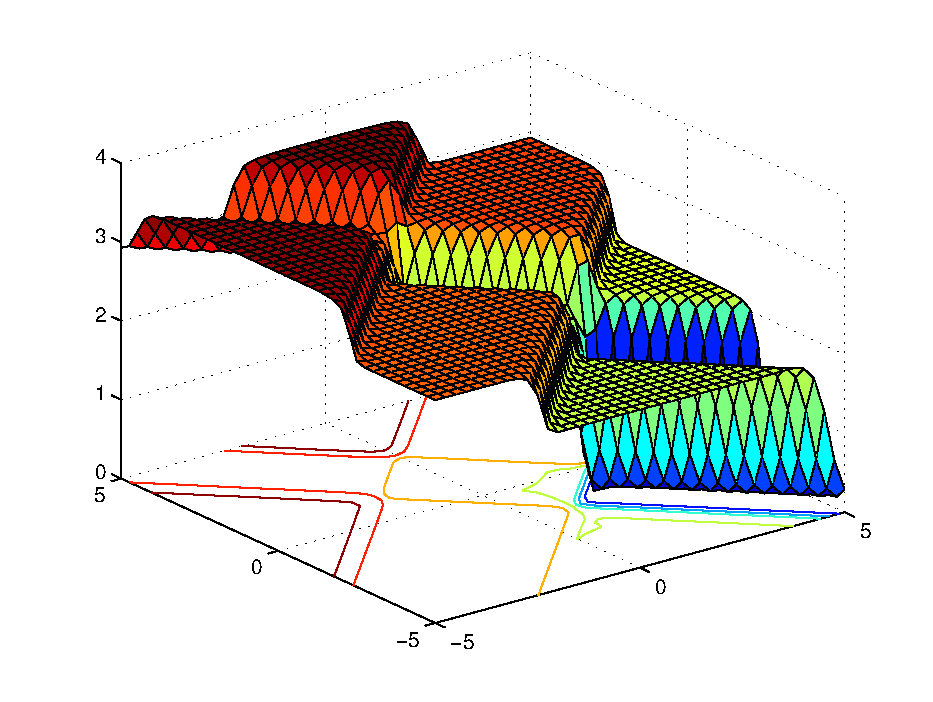
\includegraphics[width=6cm]{pics/xor_in2_10hidden}

$E(w^{(1)})$
\end{frame}






\begin{frame}
\frametitle{a great solution from 1992\dots}
\pause
\centerline{\includegraphics[width=6cm]{pics/SVM-neural.pdf}}
\end{frame}

\begin{frame}
\frametitle{a great solution from 1992?}

But: SVMs are slow (as the number of kernels increases)

\vskip1cm

Solutions:
\begin{itemize}
\item using stochastic gradient (like neural networks)
\item learning which SV to use (non-convex) (like neural networks)
\item using linear SVMs (back to the perceptron)
\end{itemize}
\end{frame}



\begin{frame}
\frametitle{on multiple hidden layers}

Insufficiently deep architectures can be exponentially inefficient.

Functions compactly represented with $k$ layers may require
exponential size with $k-1$ layers.

Multiple levels of latent variables allow combinatorial sharing
of statistical strength. 
Different tasks can share the same  features

\vspace{2cm}
\footnotesize{from:
\emph{Understanding and Improving Deep Learning Algorithms},
Yoshua Bengio, ML Google Distinguished Lecture, 2010}
\end{frame}

\begin{frame}
\frametitle{Feature Sharing}

Different high-level features can be built from the 
same set of lower-level features
\footnotesize{(from:
\emph{Understanding and Improving Deep Learning Algorithms},
Yoshua Bengio, ML Google Distinguished Lecture, 2010)}
\begin{center}
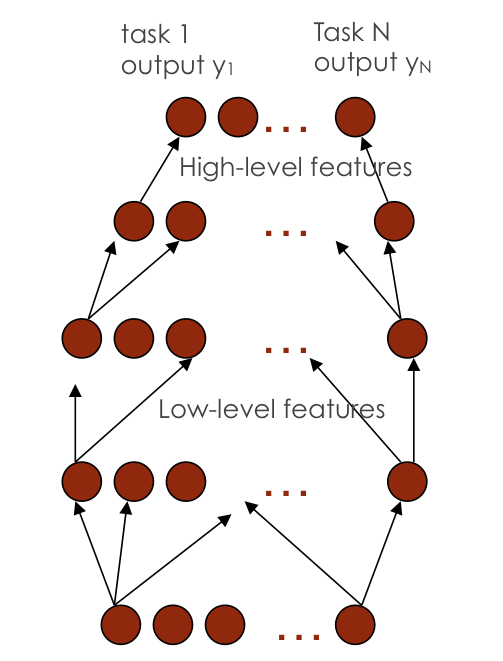
\includegraphics[width=0.5\textwidth]{pics/bengio1.png}
\end{center}
\end{frame}



\begin{frame}
\frametitle{BP problems for deep networks}

\begin{itemize}
\item requires many labeled training data \\
	\textcolor{white}{(yet since 1995 we much bigger labeled data sets)}
\item learning time does not scale well for multiple hidden layers\\
	\textcolor{white}{(and computers became MUCH faster)}
\item initialising weights is important \\
	\textcolor{white}{(so new methods were developed)}
\end{itemize}
\end{frame}


\begin{frame}
\frametitle{BP problems for deep networks}

\begin{itemize}
\item requires many labeled training data \\
	(yet since 1995 we much bigger labeled data sets)
\item learning time does not scale well for multiple hidden layers\\
	 (and computers became MUCH faster)
\item initialising weights is important \\
	(so new methods were developed)
\end{itemize}
\end{frame}




\begin{frame}
\frametitle{way out}
(It seems that)
Back-propagation breaks down for multiple hidden layers due to the vanishing gradient.

\vspace{1cm}

Recent research [Hinton et al., 2006] uses 
\emph{unsupervised pre-training} by Restricted 
Boltzmann Machines to get into vicinity of the minimum.

\vspace{1cm}

Various kinds of unsupervised pre-training:
\begin{itemize}
\item RBM (Restricted Boltzmann Machines)
\item (tied) Autoencoders and variants (denoising AE, sparse AE)
\item Sparse coding
\item \dots
\end{itemize}
\end{frame}


\begin{frame}
\frametitle{restricted Boltzmann machine}
Start by learning a generative model of the input data that has one layer of latent variables
\vskip1cm
\centerline{\includegraphics[width=6cm]{pics/RBM.pdf}}

Then use the vector of latent variable activities as data for training a second generative model.

\end{frame}


\begin{frame}
\frametitle{restricted Boltzmann machine}
for a hidden unit $h$ and a visible unit $v$ (bias $b$, weight $w$) we compute
$$
P(h_j = 1 \mid v) = \sigma \bigl(b_j + \sum_{i=1}^m w_{i,j} v_i \bigr), \quad  \textrm{$\sigma$ is sigmoid function}
$$
$$
P(v_i= 1 \mid h) = \sigma \bigl(a_i + \sum_{j=1}^n w_{i,j} h_j \bigr), \quad  \textrm{\textcolor{white}{,s is sigmoid function}}
$$
we optimise
$
\argmax_W \prod_{v \in V} P(v)
$
e.g.\ using contrastive divergence:
\pause
\centerline{\includegraphics[width=6cm]{pics/contrastivedivergence.png}}

\end{frame}


\begin{frame}
\frametitle{pretraining with RBMs}
We can combine the stack of generative models into one.  We can prove that adding a layer results in a lower bound on the log probability of the training data.

Then add an output layer, and train the stack with back propagation.
\end{frame}


\begin{frame}
\frametitle{loose remarks}

In fact, learning with enough labeled data and initialise weights with the right scales also works


These methods were initially used for speech recognition (30\% better)


In computer vision the methods  initially only used tiny datasets.  That works for few parameters or hand-engineering features; Used in google+

Trick: make early layers convolutional

Trick: take a patch of the image and move it around on the image 

Trick: use rectified linear units $\max(0,x)$ or $\log(1+e^x)$ $\longrightarrow$

Trick: dropout $\longrightarrow$

\end{frame}


\begin{frame}
\frametitle{rectifier linear units}

Here is a trick to make logistic neurons more powerful, but keeping the number of parameters constant:
\begin{enumerate}
\item make many copies of each neuron
\item all neurons have the same parameters, but have a fixed offset to the bias: $-1$, $-0.5$, $0.5$, \dots
\end{enumerate}

\vskip 1cm
\centerline{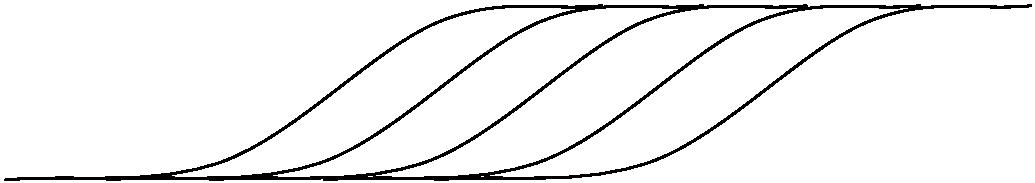
\includegraphics[width=6cm]{pics/sumlog.pdf}}
\end{frame}


\begin{frame}
\frametitle{rectifier linear units}
but
\vskip-1cm
\begin{tabular}{ccc}
{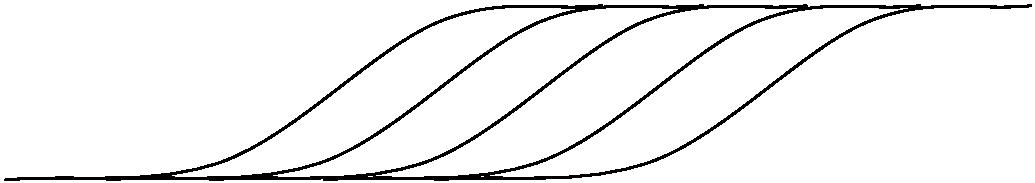
\includegraphics[width=5cm]{pics/sumlog.pdf}}
&=&
{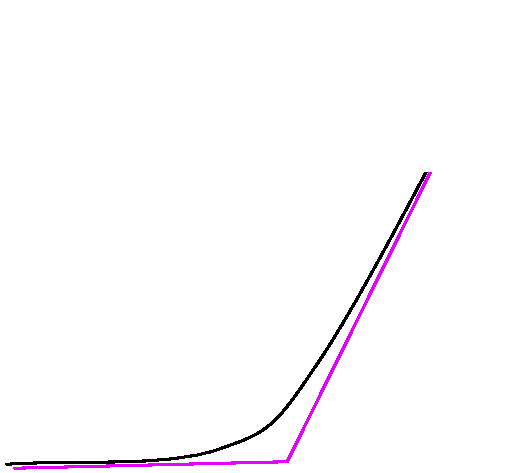
\includegraphics[width=3cm]{pics/rect.pdf}}
\\
&&\\
$\sum_{n=1}^\infty \mathrm{logistic}(x + 0.5 - n)$
&$\approx$&
$\log(1 + e^x)$
\end{tabular}
\vskip1cm
Advantages:
\begin{itemize}
\item reduces vanishing gradient.
\item  can be used in RBM to approximate real-valued inputs.
\end{itemize}
\end{frame}


\begin{frame}
\frametitle{dropout}
Let's look at a neural network with one hidden layer.

Each time a learning sample is learned, we randomly put to 0 each hidden unit with probability 0.5.

\centerline{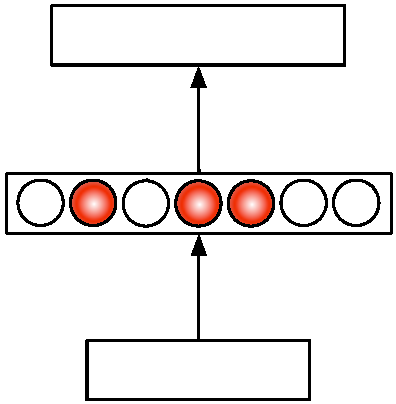
\includegraphics[width=4cm]{pics/dropout.pdf}}

We are therefore randomly sampling from $2^H$ different architectures, but these share the same weights.
\end{frame}
\begin{frame}
\frametitle{dropout $\rightarrow$ regularisation}
with $H$ hidden units, we sample from $2^H$ models---most of them are not trained! 

Weight sharing means strong regularisation.

It is much better than L1 or L2 regularisation which pull the weights to 0; instead, it pulls the weights to what other models want.

\end{frame}

\begin{frame}
\frametitle{dropout}
To compute the output, one could average all possible models.

That is too expensive, however.   Instead we take the half of the outgoing weights to get the same results.

This exactly computes the geometric mean of the predictions of all $2^H$ models.
\end{frame}


\begin{frame}
\frametitle{final remarks}
trick: if your deep neural network is overfitting, use dropout.  If it isn't, it will probably be too small!

A silly note about the brain with $10^{12}$ connections: A long life lasts $2\cdot10^9$ seconds

Theano     (Python     CPU/GPU)     mathematical     and     deep     learning
library     http://deeplearning.net/software/theano



Concerns:


   *many hyperparameters
   *many algorithms
   *non-convex optimisation
   *how do we represent model knowledge?

but


   *well parallelisable
   *simple implementation
   *beat many benchmarks
\end{frame}








\begin{frame}
\frametitle{convolutional deep learning example (Ng 2009)}
\begin{center}
first layer (top) and second layer (bottom) weights for selected images 
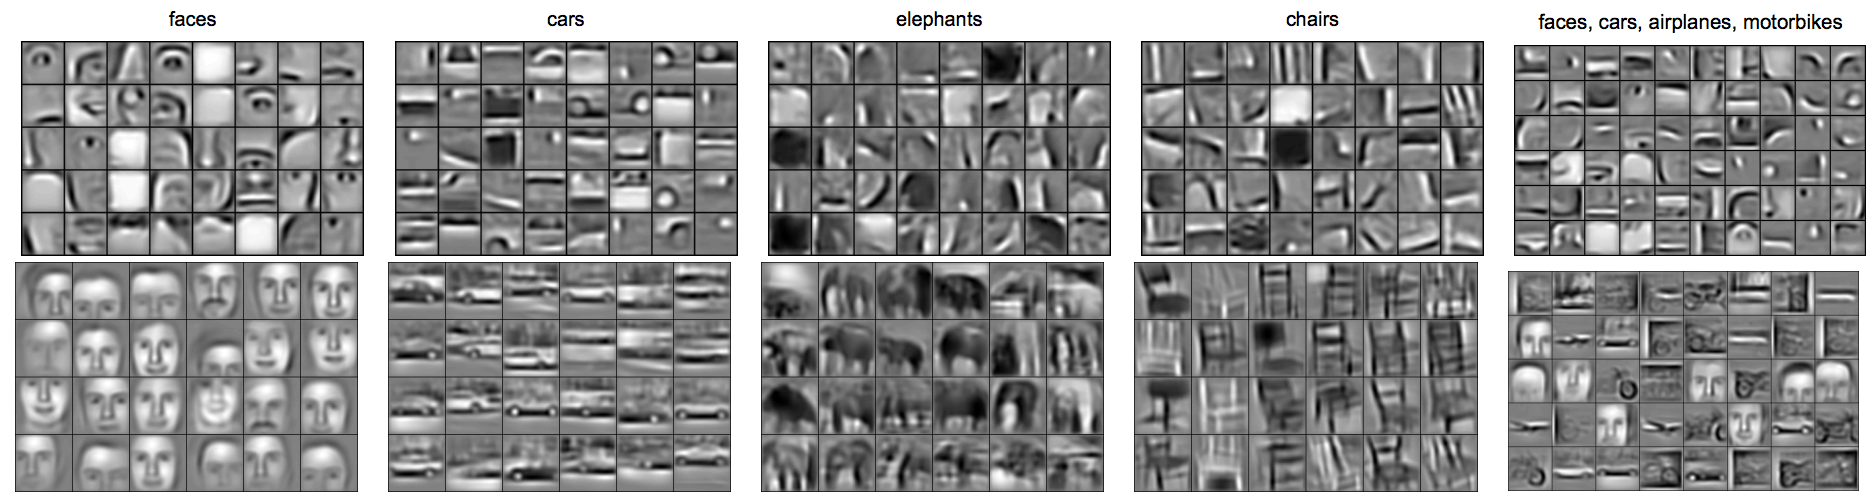
\includegraphics[width=0.99\textwidth]{pics/ng2009-1.png}

 for natural images \\
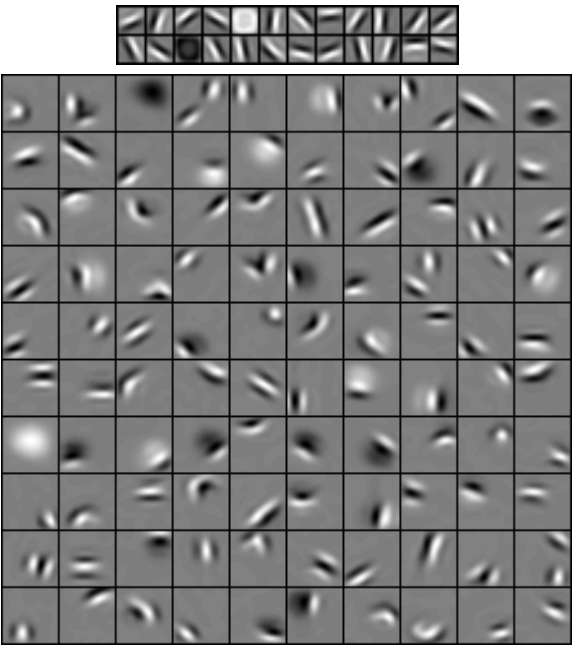
\includegraphics[height=4cm]{pics/ng2009-2.png}
\end{center}
\end{frame}



\begin{frame}
\frametitle{Deep autoencoder Example: Face Compression}
\begin{center}
\includegraphics[width=0.9\textwidth]{pics/hinton1.png}
\end{center}
\end{frame}
%%
\begin{frame}
\frametitle{Deep autoencoder Example: Text Categorisation}
\begin{center}
\includegraphics[width=0.99\textwidth]{pics/hinton2.jpg}
\end{center}
\end{frame}






\begin{frame}
\frametitle{neuroscience analogies :-/}
\vskip5mm
\centerline{\includegraphics[width=6cm]{pics/neuronentypen.png}}

Obvious conclusion:
human cortex has 6 layers.
You will find Reichardt detectors in V1.   Yet
%hippocampus: place cells
\begin{itemize}
\item ``spiking version'' of BP?
\item single cells in the medial temporal lobe representing complex concepts: gender, facial expression, \dots
\item but also movement ``primitives''
\item cells coding multimodal invariant things, faces, categories\dots e.g.\ Halle Berry cell; Jennifer Aniston cell; Sydney Opera House cell
\item dendrites are active, change the data, can generate spikes.
\end{itemize}


\end{frame}



%\frame{\frametitle{the transfer function}
%  \begin{columns}
%    \begin{column}{5.0cm}
%The response of a simulated neuron to its activation $a_j$ is given by a \alert{transfer function}
%$$
%o_j = \phi_j(a_j)
%$$
%\vfill
%    \end{column}
%    \begin{column}{4.0cm}
%			\hfill\imgbox{trafctneuron}{}{4.0cm}
%		\end{column}
%  \end{columns}
%
%In the simplest case, the transfer function can be selected to be the identity function, or another linear function. However, in order for the network to exhibit nonlinear properties, $\phi(\cdot)$ also has to be nonlinear.
%}
%
%\frame{\frametitle{the transfer function}
%\begin{itemize}
%	\item historically, binary and piecewise linear transfer functions were
%		chosen first, in reference to the threshold-like behaviour of biological neurons
%	\pause
%	\item smooth, S-shaped (=\alert{sigmoid}) functions behave like
%		threshold or linear functions, depending on scaling, and can be differentiated
%	\pause
%	\item another network class, radial basis function (RBF) networks,
%		uses Gaussian-shaped transfer functions.
%\end{itemize}
%
%}
%
%\frame{\frametitle{commonly used transfer functions}
%\imgbox{transferfct}{}{\textwidth}
%}
%

%%%%
%\begin{frame}[fragile]
%\frametitle{better algorithm for backprop (``(mini) batch learning'')}
%
%\begin{beamerboxesrounded}[upper=def,lower=block body,width=1.03\textwidth,shadow]{\textbf{back-propagation algorithm:}}
%\begin{lstlisting}[mathescape]
%initialise the weights
%repeat
%  randomly select samples $(\bfx,\bfz)$ from a mini-batch do
%  begin
%     $\bf o = \cl M(\bfw, \bfx)$; forward pass
%     calculate error $\bfz  - \bf o$ at the output units
%     for all $w^{(2)}$ compute $\delta_{w^{(2)}}$; backward pass
%     for all $w^{(1)}$ compute $\delta_{w^{(1)}}$; backward pass continued
%     sum the delta weights using $\partial E / \partial w_{ij} = \delta_{j} x_{i}$
%  end
%  update the weights using summed delta weights
%until stopping criterion satisfied
%\end{lstlisting}
%\end{beamerboxesrounded}
%\end{frame}

%%%%%%%%%%%%%%




%\begin{frame}
%\frametitle{Minkowski-R error }
%We previously assumed Gaussian distribution of the target values by
%$$
%p(\epsilon) = { 1 \over \sqrt{2\pi\sigma^2}} \exp\left(-{\epsilon^2\over 2 \sigma^2}\right)
%$$
%\pause
%If we take the more general form
%$$
%p(\epsilon) = { R \beta^{1/R} \over 2 \Gamma (1/R)} \exp\left(-\beta |\epsilon|^R\right)
%$$
%The likelihood of the prior leads to minimisation of 
%$$
% E(\bfw) = {1 \over 2} \sum _{p=1}^{n} \left|\bfz_{p} - \cl M(\bfw, \bfx_{p})\right|^R
% $$
%\end{frame}

%%%%%%%%%%%  some ``new'' stuff for classifiers

%\begin{frame}
%\frametitle{FFNN for classification}
%Take a set of classification data $\mathcal C_0 = \{(\bfx, z=0)\}$ and  $\mathcal C_1 = \{(\bfx, z=1)\}$
%
%If we take an FFNN with sigmoidal outputs
%$$
%y = \phi(a) = {1 \over 1 + \exp(-a)}
%$$
%we can interpret the output $y(\bfx, \bfw)$ as the conditional
%probability $p(\mathcal C_0 \mid \bfx)$ while $p(\mathcal C_1 \mid \bfx) = 1-y(\bfx,\bfw)$.
%
%\pause
%But then the likelihood is a Bernoulli distribution
%$$
%p(t \mid \bfx, \bfw) = y(\bfx, \bfw)^z \bigl[1-y(\bfx,\bfw)\bigr]^{1-z}
%$$
%\pause
%The negative log likelihood then leads to
%$$
%E(\bfw) = -\sum_{p=1}^n \Bigl\{
%	z_p \log y(\bfx_p, \bfw) + (1 - z_p) \log \bigl[1 - y(\bfx_p, \bfw)\bigl]
%	\Bigr\}
%$$
%Has been shown to lead to better results!
%\end{frame}





\frame{\frametitle{auto-encoder networks}
\ParBeg{idea:} find compact representation of inputs (unsupervised!)\ by
\begin{enumerate}
	\item letting the network re-create its own inputs, i.e., $\Vec{z}_n\equiv\Vec{x}_n$, and
	\item creating a bottleneck by using fewer hidden units than inputs.
\end{enumerate}
\medskip

\begin{columns}
\column{0.4\textwidth}
\imgbox{autoenc}{}{\textwidth}
\column{0.4\textwidth}
\begin{itemize}
	\item \alert{activations of hidden units} = compact code for $\Vec{x}$
	\item usually many ways of encoding the same input and output
\end{itemize}
\end{columns}
These networks make a compact representation of data (``dimensionality reduction'').
However, you cannot control the representation!

\pause
\bf Caveat: autoencoders do little more than PCA! $\rightarrow$ deep autoencoders
}



%
%\begin{frame}
%\frametitle{Very recent developments}
%Deep Learning via Hessian-Free optimisation (J. Martens, ICML 2010)---add a regularisation
%term to the Hessian, i.e., $B=H+\lambda I$
%
%%Krylov Subspace Descent for Deep Learning (O. Vinyals and D. Povey, AISTATS 2012)
%
%Deep learning also works by training ordinary backprop ``ad infinitum'' 
%on \textsl{many} data (Cire\c san et al, 2010)---extend mnist by adding
%linearly convoluted versions of the images
%\end{frame}




\end{document}
